\documentclass[12pt]{ctexart}
    %%% Document Settings %%%%
%\usepackage[utf8]{inputenc}

\usepackage[
    twoside,
    top=1in,
    bottom=0.75in,
    inner=0.5in,
    outer=0.5in,
]{geometry}
\pagestyle{myheadings}
\usepackage{minted}
\usepackage[dvipsnames,svgnames]{xcolor}

%%%% Additional Commands to Load %%%%
\usepackage{tcolorbox}
\tcbuselibrary{skins}
\tcbuselibrary{minted}
\usemintedstyle{lovelace}
%\usepackage{minted}
\usepackage{color}
\usepackage{tikz}
\usetikzlibrary{calc}
\usepackage{tabularx,colortbl}
\usepackage{amsfonts,amsmath,amssymb}
\usepackage{titling}
\usepackage{mathrsfs}
\usepackage{calc}
\usepackage{subcaption}

\usepackage{listings}
%\usepackage{newtxtext}
\usepackage[strict]{changepage} 
\usepackage{framed}
\definecolor{formalshade}{rgb}{0.95,0.95,1}
\usepackage{float}

%%%% Commands to Define Homework Boxes %%%%
%%%% Box Definition %%%%
\newtcolorbox{prob}[1]{
% Set box style
    sidebyside,
    sidebyside align=top,
% Dimensions and layout
    width=\textwidth,
    toptitle=2.5pt,
    bottomtitle=2.5pt,
    righthand width=0.20\textwidth,
% Coloring
    colbacktitle=gray!30,
    coltitle=black,
    colback=white,
    colframe=black,
% Title formatting
    title={
        #1 \hfill Grade:\phantom{WWWW}
    },
    fonttitle=\large\bfseries
}

%%%% Environment Definition %%%%
\newenvironment{problem}[1]{
    \begin{prob}{#1}
}
{
    \tcblower
    \centering
    \textit{\scriptsize\bfseries Faculty Comments}
    \vspace{\baselineskip}
    \end{prob}
}

\newenvironment{formal}{%
\def\FrameCommand{%
\hspace{1pt}%
{\color{DarkBlue}\vrule width 2pt}%
{\color{formalshade}\vrule width 4pt}%
\colorbox{formalshade}%
}%
\MakeFramed{\advance\hsize-\width\FrameRestore}%
\noindent\hspace{-4.55pt}% disable indenting first paragraph
\begin{adjustwidth}{}{7pt}%
\vspace{2pt}\vspace{2pt}%
}
{%
\vspace{2pt}\end{adjustwidth}\endMakeFramed%
}

    \title{特殊方程作业9}
    \author{地物2201班\ 杨曜堃}
    \date{\today}
%%% document
\begin{document}

% Format Running Header
    \markboth{\theauthor}{\thetitle}
    \maketitle
    \begin{description}
        \item[问题1] 采用傅里叶变换法求解下列热传导方程的定解问题:$$
        \begin{cases}
            \dfrac{\partial u}{\partial t}=\dfrac{\partial^2u}{\partial x^2},\quad -\infty<x<+\infty,\ t>0\\
            u(x,0)=\varphi(x)=\begin{cases}
                \frac{1}{2a},& |x|\leqslant a\\
                0,& |x|>a,\ a>0
            \end{cases}\\
            \lim_{|x|\to\infty}u(x,t)=0
        \end{cases}
        $$
        要求:图示$t=1$、$a=1,3,5$时的计算结果。
    \end{description}
    \begin{problem}{问题\#1}
        首先对$u$进行关于$x$的傅里叶变换$$
        \mathscr{F}\left\{u(x,t)\right\}=U(\omega,t)=\int^{+\infty}_{-infty}u(x,t)e^{-j\omega t}\text{d}x$$
        根据傅里叶变换的微分性质$$
        \mathscr{F}\left\{\dfrac{\partial^2 u}{\partial x^2}\right\}=(j\omega)^2U(\omega,t)=-\omega^2U(\omega,t)
        $$
        同理做关于$t$的傅里叶变换$$
        \mathscr{F}\left\{\dfrac{\partial u}{\partial t}\right\}=\int^{+\infty}_{-\infty}e^{-j\omega x}\text{d}u(x,t)e^{-j\omega x}\text{d}x=\dfrac{\text{d}U}{\text{d}t}
        $$
        对$\varphi(x)$做傅里叶变换,由于是方波,无需查表便可推导其傅里叶变换
        $$
        \mathscr{F}\left\{\varphi(x)\right\}=\varPhi(\omega)=\int^{+\infty}_{-\infty}\varphi(x)e^{-j\omega x}\text{d}x
        $$
    \end{problem}
    \begin{problem}{问题\#1}
        被积函数在$(-\infty,-a)$和$(a,+\infty)$上为0,可以改写积分 上下限
        $$
        \begin{aligned}
            \varPhi(\omega)&=\int^{a}_{-a}\dfrac{1}{2a}e^{-j\omega x}\text{d}x\\
            &=-\dfrac{1}{2ja\omega}\left[e^{-ja\omega}-e^{ja\omega}\right]\\
            &=\dfrac{\sin a\omega}{a\omega}
        \end{aligned}
        $$
        因此,定解问题可以转变为
        $$
        \begin{cases}
            \dfrac{\text{d}U}{\text{d}t}+\omega^2U(\omega,t)=0\\
            U(\omega,0)=\varPhi(\omega)
        \end{cases}
        $$
        求解常微分方程得到通解$$
        U(\omega,t)=A(\omega)e^{-\omega^2t}$$
        代入初始条件可得
        $$A(\omega)=\varPhi(\omega)$$
        即频域上的解
        $$U(\omega,t)=\varPhi(\omega)e^{-\omega^2t}$$
        此时还需要对$U(\omega,t)$做傅里叶逆变换,注意到该频域上的解是两函数相乘的形式。根据傅里叶变换的卷积性质可知,$u(x,t)$应该是两函数对应逆变换的卷积形式,并且显然有
        $$\mathscr{F}^{-1}\left\{\varPhi(\omega)\right\}=\varphi(x)$$
        所以只需关注高斯函数的傅里叶逆变换,可以证明高斯函数的傅里叶变换任然是高斯函数(高斯函数是傅里叶变换的特征函数)。证明如下
        \begin{formal}
            设$f(x)=e^{-\pi x^2}$,定义
            $$
            F(\omega)\triangleq\mathscr{F}\left\{f(x)\right\}=\int^{+\infty}_{-\infty}e^{-\pi x^2}e^{-j\omega x}\text{d}x
            $$
            为了满足归一化条件,需要将角频率$\omega$转换成自然频率$\xi$
        \end{formal}
    \end{problem}
    \begin{problem}{问题\#1}
        \begin{formal}
            $$
            F(\xi)=\int^{+\infty}_{-\infty}e^{-\pi x^2}e^{-2njx\xi}\text{d}x
            $$
            显然有$F(0)=1$,$f'(x)=-2\pi xf(x)$。对$F(\xi)$求导,利用先导后积的性质
            $$
            \begin{aligned}
                F'(\xi)&=\int^{+\infty}_{-\infty}(-2\pi jx)f(x)e^{-2\pi jx\xi}\text{d}x\\
                &=j\int^{+\infty}_{-\infty}f'(x)e^{-2\pi jx\xi}\text{d}x
            \end{aligned}
            $$
            结合傅里叶变换的微分性质,得到微分方程
            $$
            F'(\xi)=j\mathscr{F}\left\{f'(x)\right\}=j(2\pi j\xi)F(\xi)=-2\pi\xi F(\xi)
            $$
            定义$G(\xi)\triangleq e^{\pi\xi^2}F(\xi)$,对$G(\xi)$求导并代入微分方程
            $$
            \begin{aligned}
                G'(\xi)&=2\pi\xi e^{\pi\xi^2}F(\xi)+e^{\pi\xi^2}F'(\xi)\\
                &=2\pi\xi e^{\pi\xi^2}F(\xi)-2\pi\xi e^{\pi\xi^2}F(\xi)\\
                &=0
            \end{aligned}
            $$
            所以$G(\xi)$应该为一个常数,由于$F(0)=1$,所以$G(\xi)\equiv 1$。因此可得$F(\xi)=e^{-\pi\xi}$
            即
            $$
            \mathscr{F}\left\{e^{-\pi x^2}\right\}=e^{-\pi\xi^2}
            $$
            证毕。
        \end{formal}
        这一性质提供了一种便利性,而本题所关注的$e^{-\omega^2t}$可以看作是对标准高斯函数做伸缩变换得到的。根据结论,不妨计算$e^{-ax^2}$的傅里叶变换,记
        $$
        I=\int^{+\infty}_{-\infty}e^{-ax^2}e^{-j\omega t}\text{d}t
        $$
        利用分部积分法
        $$
        \begin{aligned}
            I&=\dfrac{j}{\omega}\int^{+\infty}_{-\infty}e^{-ax^2}\text{d}e^{-j\omega x}
            =\dfrac{j}{\omega}\left(0-\int^{+\infty}_{-\infty}e^{-j\omega x}\text{d}e^{-ax^2}\right)\\
            &=\dfrac{2ja}{\omega}\int^{+\infty}_{-\infty}xe^{-ax^2}e^{-j\omega x}\text{d}x\\
            &=\dfrac{2ja}{\omega}\mathscr{F}\left\{xe^{-ax^2}\right\}\\
        \end{aligned}
        $$
    \end{problem}
    \begin{problem}{问题\#1}
        利用傅里叶变换微分性质的对偶性质
        $$
        I=-\dfrac{2a}{\omega}\dfrac{\text{d}I}{\text{d}\omega}
        $$
        解该微分方程可得
        $$
        I(\omega)=I(0)e^{-\frac{\omega^2}{4a}}
        $$
        很显然
        $$
        I(0)=\int^{+\infty}_{-\infty}e^{-ax^2}\text{d}x=\sqrt{\dfrac{\pi}{a}}
        $$
        得到
        $$
        \mathscr{F}\left\{e^{-ax^2}\right\}=\sqrt{\dfrac{\pi}{a}}\ e^{-\frac{\omega^2}{4a}}
        $$
        用$\dfrac{1}{4a}$替换$a$,可以得到
        $$
        \mathscr{F}\left\{e^{-\frac{x^2}{4a}}\right\}=2\sqrt{a\pi}e^{-a\omega^2}
        $$
        再由傅里叶变换的线性性质可得
        $$
        \mathscr{F}\left\{\dfrac{1}{2\sqrt{a\pi}}e^{-\frac{x^2}{4a}}\right\}=e^{-a\omega^2}
        $$
        利用该傅里叶变换对,得出$e^{-\omega^2t}$的傅里叶逆变换
        $$
        \mathscr{F}^{-1}\left\{e^{-\omega^2t}\right\}=\dfrac{1}{2\sqrt{\pi t}}e^{-\frac{x^2}{4t}}
        $$
        因此定解问题的解为
        $$
        u(x,t)=\dfrac{1}{2\sqrt{\pi t}}\int^{+\infty}_{-\infty}e^{-\frac{(x-\xi)^2}{4t}}\varphi(\xi)\text{d}\xi
        $$
        进一步计算得到
        $$
        u(x,t)=\dfrac{1}{4a\sqrt{\pi t}}
        \int^{a}_{-a}e^{-\frac{(x-\xi)^2}{4t}}\text{d}\xi
        $$
        该积分项为非初等函数,令$z=\dfrac{\xi-x}{2\sqrt{t}}$,$\text{d}z=\dfrac{1}{2\sqrt{t}}\text{d}\xi$,结果可以改写为
        $$
        u(x,t)=\dfrac{1}{2a\sqrt{\pi}}\int^{\frac{a-x}{2\sqrt{t}}}_{\frac{-a-x}{2\sqrt{t}}}e^{-z^2}\text{d}z
        $$
    \end{problem}
    \begin{problem}{问题\#1}
        利用误差函数
        $$
        \text{erf}(x)=\dfrac{2}{\sqrt{\pi}}\int^{x}_{0}e^{-z^2}\text{d}z
        $$
        所以有
        $$
        \begin{aligned}
            u(x,t)&=\dfrac{1}{4a}\int^{\frac{a-x}{2\sqrt{t}}}_{0}e^{-z^2}\text{d}z-\dfrac{1}{4a}\int^{\frac{-a-x}{2\sqrt{t}}}_{0}e^{-z^2}\text{d}z\\
            &=\dfrac{1}{4a}\left[
                \text{erf}\left(\dfrac{a-x}{2\sqrt{t}}\right)- \text{erf}\left(\dfrac{-a-x}{2\sqrt{t}}\right)
            \right]
        \end{aligned}
        $$
        误差函数为奇函数,从而原定解问题的解可以写成
        $$
        u(x,t)=\dfrac{1}{4a}\left[
            \text{erf}\left(\dfrac{x+a}{2\sqrt{t}}\right)- \text{erf}\left(\dfrac{x-a}{2\sqrt{t}}\right)\right]
        $$
        当$t=1$时,采用如下MATLAB代码计算$a=1,3,5$时的结果。
    \end{problem}
    \begin{lstlisting}[language = Matlab,title={test9.m},  numbers=left, 
        numberstyle=\tiny,keywordstyle=\color{blue!70},
        commentstyle=\color{red!50!green!50!blue!50},frame=shadowbox,
        rulesepcolor=\color{red!20!green!20!blue!20},basicstyle=\ttfamily]
        % 一维无限长杆热传导问题结果图示
        clear;

        x = -10:0.01:10;
        a = [1 3 5];
        for i = 1:size(a,2)
        u(i, : ) = 0.25*(erf(0.5*(x+a(i)))-erf(0.5*(x-a(i))))/a(i);
        end

        % 绘制图像
        plot(x,u);
        xlabel('x');
        ylabel('y');
        legend('a=1','a=3','a=5');
    \end{lstlisting}
    \begin{figure}[htbp]
        \small
        \centering
        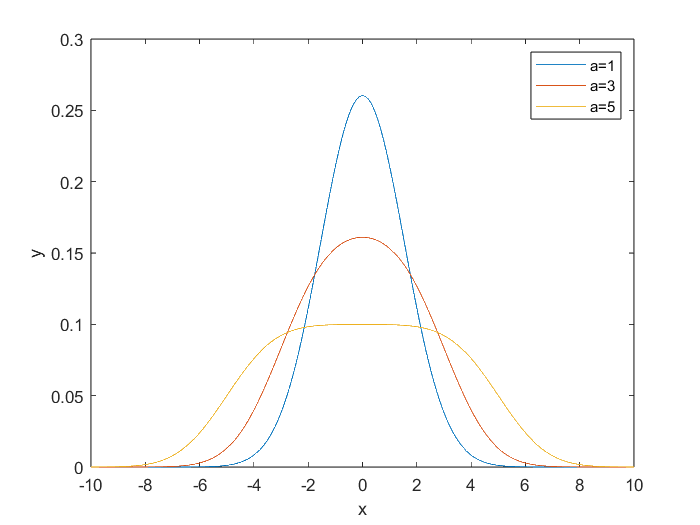
\includegraphics[width=16cm]{fig1.png}
        \caption{MATLAB计算结果图示} \label{Fig:aa}
    \end{figure}
\end{document}